\section{MariaDB mit OQGRAPH}%Graph-Datenbanken im praktischen Einsatz: OLAP (chapter)
In diesem Abschnitt wird auf die Performanz von OLAP-Anwendungen in MariaDB-Datenbanksysteme mit OQGRAPH als Erweiterung eingegangen. Als OLAP-Testszenario werden Profile aus Datensätzen verschiedener Plattformen herangezogen. Diese Profile dienen fortlaufend als Knoten. Diese Knoten werden dann in weiteren Datensätzen über Kanten miteinander verbunden. Diese Kanten beinhalten außerdem zusätzliche Informationen, wie die Art der Beziehung, sowie ein Datum.

Die Daten sind den Plattformen \emph{Facebook}, \emph{Wikipedia}, \emph{Epinions}, \emph{YouTube} und \emph{LifeJournal} zugeordnet. Die entsprechenden Datensätze beinhalten alle eine unterschiedliche Anzahl an Knoten und Kanten.

\subsection{Implementierung der Datenbanken}

Für die Performanztests von MariaDB mit der OQGRAPH-Erweiterung wird der zur Verfügung stehende Cluster genutzt. Details zur Installation von MariaDB und der OQGRAPH-Erweiterung können dem Abschnitt \ref{Installation} entnommen werden. Es wird also ein bereits bestehendes MariaDB-Datenbanksystem genutzt, welches bis hierhin nur für die Implementierung der OLTP-Anwendung genutzt wurde. Um die Performanztests nicht zu verfälschen, wurde das MariaDB-Datenbanksystem für die Dauer der Tests nicht anderweitig genutzt.

Um die Datensätze voneinander zu abstrahieren und um die Performanztests voneinander unabhängig durchzuführen, wurde für jede Plattform jeweils eine Datenbank angelegt. In den fünf Datenbanken befinden sich jeweils zwei Tabellen.

Die Tabelle \emph{profil} beinhaltet alle Profile aus den Datensätzen der jeweiligen Plattformen. Jede Zeile in der Tabelle stellt hierbei einen Knoten dar. Dabei stellt die Tabelle \emph{profil} noch weitere Informationen zum Knoten zur Verfügung, wie den Vor- und Nachnamen, das Geschlecht, das Geburtsdatum und das Land. Das Land wurde noch indexiert, welches bei den Performance Messungen zur Anwendung kommt.

In der Tabelle \emph{oq\_backing} werden die Kantenbeziehungen zwischen den einzelnen Knoten gespeichert. Dabei folgt die Tabelle der Namenskonvention der OQGRAPH-Erweiterung. Die Spalte \emph{origid} referenziert hierbei auf den Ausgangsknoten, von dem eine gerichtete Kante zum Zielknoten ausgeht, welcher in \emph{destid} referenziert wird. Außerdem werden in den Spalten \emph{rtype} und \emph{date} weitere Informationen zur Kantenbeziehung gespeichert.

Für den Import der Zeilen aus den CSV-Datensätzen in die Datenbank wurde die Datenbank-IDE DataGrip genutzt. Beim CSV-Import wandelt die DataGrip-IDE die CSV-Datei in mehrere Insert-SQL-Statements um und führt diese Statements in der ausgewählten Datenbank aus. So wurden schließlich alle Zeilen aus den CSV-Dateien in die Datenbank importiert.

Die Anzahl der Zeilen in den Tabellen der verschiedenen Datenbanken kann der folgenden Auflistung entnommen werden.

\begin{center}
	\begin{tabular}{l|l l l l l }
		& Facebook & Wikipedia & Epinions & YouTube & LifeJournal \\
		\hline
		profil & 4.039 & 7.115 & 75.879 & 1.134.890 & 3.997.962 \\
		oq\_backing & 88.234 & 100.762 & 405.740 & 2.987.624 & 34.681.189 \\
	\end{tabular}
\end{center}

\subsection{Versuchsaufbau und Metriken}

Im Rahmen des Performanztests wird die Dauer einer einzelnen Operation als Metrik herangezogen. Hierbei wird die Zeit gemessen, die eine Operation in Form eines SQL-Statements benötigt. Hierbei kann es aber auch zu ausreißenden Beobachtungen kommen. Ausreißer können entstehen, weil das MariaDB-Datenbanksystem eine SQL-Abfrage nicht immer gleich und deshalb diese nicht immer über eine konstant gleichbleibende Dauer ausführt.

Es ist daher wichtig den Einfluss von Ausreißern möglichst zu minimieren. Aus diesem Grund werden die Messungen mehrmals durchgeführt und anschließend der durchschnittliche Zeitbedarf berechnet. Je nach Zugriffsart finden weitere Messungen statt. So werden bei Projektionen und Selektionen unterschiedliche Stellen der Tabellen abgefragt, da Abfragen auf den Beginn oder das Ende der Tabelle die Messungen verfälschen würde.

Die Mess-Vorgänge wurden in SQL-Prozeduren definiert. Diese Prozeduren übernehmen die Zeitmessung, die Speicherung der Messwerte, sowie die Ermittlung des Durchschnittes. Die Messergebnisse werden dabei in einer weiteren Tabelle \emph{analysis} gespeichert, die auf jeder Datenbank erstellt wurde. Die Prozeduren werden dann mittels des \emph{CALL}-SQL-Befehls aufgerufen.

\subsection{Annahmen}

\subsection{Performance-Messung}

\subsubsection{Projektion und Selektion}
Da OQGRAPH lediglich die Traversierung von Knoten ermöglicht sind die in diesem Kapitel durchgeführten Leistungstests keine Evaluierung des Graphsystems sondern der darunterliegenden relationalen Datenbank. Ein Ansatz, den Zugriff nur über die Kantentabelle zu ermöglichen, um so einen Anbindung an OQGRAPH zu simulieren wurde verworfen. Da die Performance unnötig leiden würde, da die Datenknotentabelle in jedem Fall gejoined werden muss. Gleichzeitig gibt es auch keine Vorteile, da der Primary Key der Datentabelle mit dem Knotenwert in der Backingtabelle identisch ist. Des Weiteren könnten die Ergebnisse verfälscht werden, wenn ein Datensatz kein Bestandteil einer Beziehung ist, sprich es existiert keine Kante zu diesem Datensatz.

Bei der Selektion anhand von Primärschlüsseln wurde eine Messung mit dem erstem (ID = 1) Datensatz durchgeführt. Es folgend weitere Messungen in tausender Schritten (ID + 1000) bis das Ende der Tabelle erreicht wird. So lässt sich sicherstellen das dass das Mittelmaß der Messungen auch realistisch ist.

Folgende \lstinline{SELECT} Statements wurden ausgeführt:
\begin{lstlisting}
-- Nur der Primaerschlussel
SELECT id FROM profil WHERE id = x;
-- Das Vollstaendige Profil
SELECT * FROM profil WHERE id = x;
\end{lstlisting}

Abbildung \ref{fig:NutzerPk} zeigt die Ergebnisse auf den unterschiedlichen Datenbanken. Es lassen sich nur leichte Schwankungen bei den Messwerten feststellen. Die Größe der Datenbank ist daher eher unerheblich, tendenziell benötigen Selektion mit sämtlichem Attributen mehr Zeit, ist aber durchaus vernachlässigbar.
\begin{figure}[h]
	\centering
	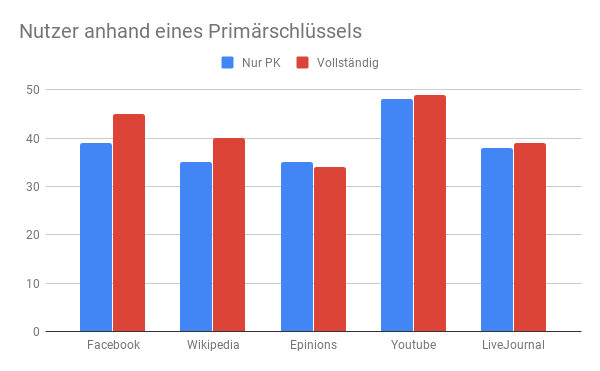
\includegraphics[width=\textwidth]{images/NutzerPk.png}
	\caption{Messergebnisse zur Selektion eines Nutzers anhand des Primärschlüssels}
	\label{fig:NutzerPk}
\end{figure}

Bei der Selektion anhand eines Nichtprimärschlüssels offenbarten sich zwei Probleme. Da auf den selektierten Attributen kein \emph{Unique Constraint} definiert ist, benötigen große Datenbanken exponentiell länger für die selbe Anfrage, da ein kompletter Scan durchgeführt werden muss. Dementsprechend ist die Vergleichbarkeit nicht mehr gewährleistet. Dieses Problem ließ sich durch eine \lstinline{LIMIT 1} Klausel lösen.

Problematisch war auch, dass sich im Gegensatz zum Primärschlüssel die Anzahl der Abfragen nur schwer begrenzen lässt, da sich nicht mit fest vorgegeben Parameter arbeiten lässt. Stattdessen liefert ein zuvor definierter Cursor, welcher \lstinline{DISTINCT} Werte des entsprechenden Attributs selektiert, die Parameter. Im Falle des indexierten Zugriff erübrigte sich das Problem von selbst, da die Anzahl der Länder in einem idealem Rahmen lagen. Bei dem nicht indexierten Zugriff wurde aber nach den Nachnamen gesucht, hier mussten die Parameter noch weiter eingeschränkt werden. Durch die Verwendung einer \lstinline{WHERE RAND()<=0.001} Klausel konnte der Parameterraum auf ein tausendstel reduziert werden.

Bei der Selektion mittels Nichtschlüsselattributen wurden folgenden \lstinline{SELECT} Statements ausgeführt:
\begin{lstlisting}
-- Anhand eines indexierten Attributes
SELECT * FROM profil WHERE country = v LIMIT 1;
-- Anhand eines nicht-indexierten Attributes
SELECT * FROM profil WHERE last = v LIMIT 1;
\end{lstlisting}

Abbildung \ref{fig:NutzerNPk} und Abbildung \ref{fig:NutzerNPkI} zeigt die Ergebnisse der nicht-indexierten und indexierten Selektion auf den unterschiedlichen Datenbanken. Es ist zu erkennen das bei einer Selektion die Performanz von sehr großen Datenbank stark leidet. Auch bei einem indexierten Zugriff nimmt die Performanz mit steigender Datenmenge ab, die benötigte Zeit ist aber dennoch wesentlich geringer.
\begin{figure}[h]
	\centering
	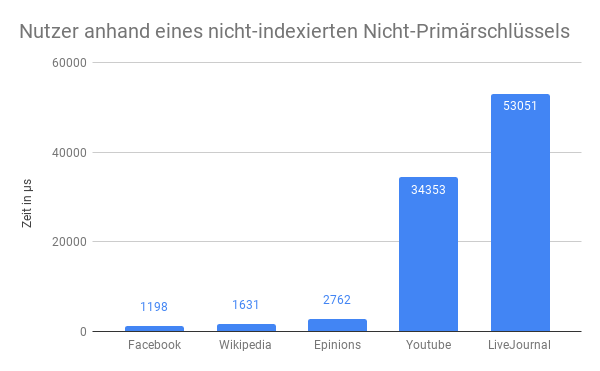
\includegraphics[width=\textwidth]{images/NutzerNPk.png}
	\caption{Messergebnisse zur Selektion eines Nutzers anhand eines Nicht-Primärschlüssels}
	\label{fig:NutzerNPk}
\end{figure}

\begin{figure}[h]
	\centering
	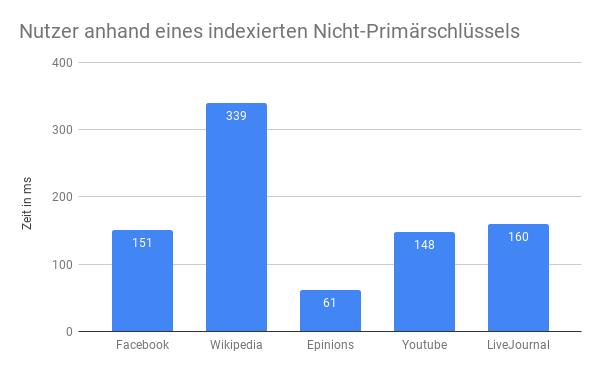
\includegraphics[width=\textwidth]{images/NutzerNPkI.png}
	\caption{Messergebnisse zur Selektion eines Nutzers anhand eines Nicht-Primärschlüssels}
	\label{fig:NutzerNPkI}
\end{figure}


\subsubsection{Aggregation}
Aus dem selben Grund wie bei Selektion und Projektion wurden auch bei diesen Tests ledigliche die relationalen SQL Datentabellen betrachtet.

Folgende Tests wurden durchgeführt:
\begin{enumerate}
	\item Anzahl aller Nutzer - Abbildung \ref{fig:AnzahlNutzer}
	\item Anzahl aller Beziehungen zwischen Nutzern - Abbildung \ref{fig:AnzahlBeziehung}
	\item Durchschnittliche Alters aller Nutzer - Abbildung \ref{fig:DurschAlter}
	\item Durchschnittliche Dauer aller Beziehung - Abbildung \ref{fig:DurschBeziehung}
\end{enumerate}

Folgende SQL Statements wurden durchgeführt:
\begin{lstlisting}
-- Anzahl Nutzer
SELECT COUNT(id) FROM profil;
-- Anzahl Beziehungen
SELECT COUNT(*) FROM oq_backing;
-- Durchschnittsalter
SELECT AVG(YEAR(NOW()) - YEAR(birth)) FROM profil;
-- Durchscnittsdauer Beziehungen
SELECT AVG(DATEDIFF(CURRENT_DATE, date)) FROM oq_backing;
\end{lstlisting}

Die Ergebnisse sind wenig überraschend, so steigt mit wachsender Datenmenge auch die benötigte Zeit. Je komplexer die Berechnung desto steiler der Anstieg. Da diese Operationen auf einer relationalen Tabelle ausgeführt wurden, machen sich auch die Vorteile eines solchen Models bemerkbar. Es ist davon auszugehen das spaltenweise SQL Aggregation wesentlich performanter ist, da nicht erst die Knoten geladen und deren Attribute extrahiert werden müssen.

\begin{figure}
	\centering
	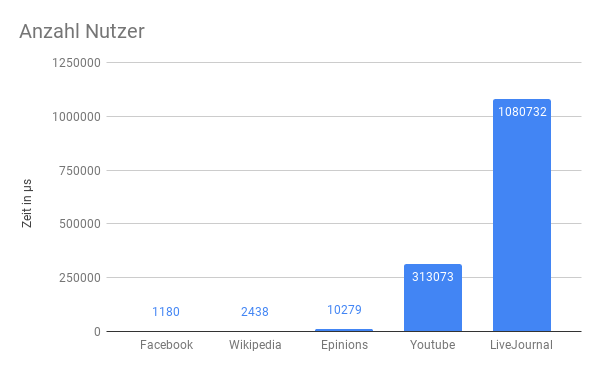
\includegraphics[width=\textwidth]{images/AnzahlNutzer.png}
	\caption{Messergebnisse zur Zählung sämtlicher Nutzeraccounts}
	\label{fig:AnzahlNutzer}
\end{figure}

\begin{figure}
	\centering
	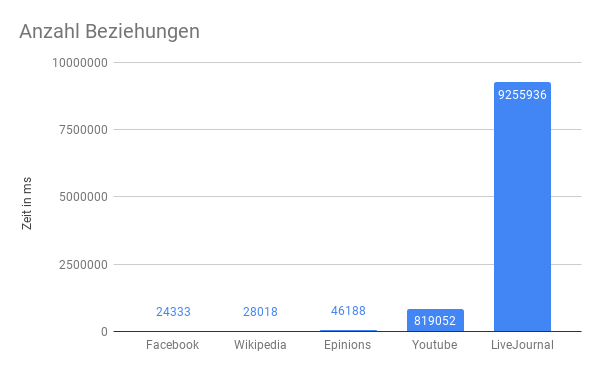
\includegraphics[width=\textwidth]{images/AnzahlBeziehung.png}
	\caption{Messergebnisse zur Zählung bestehender Beziehungen}
	\label{fig:AnzahlBeziehung}
\end{figure}

\begin{figure}
	\centering
	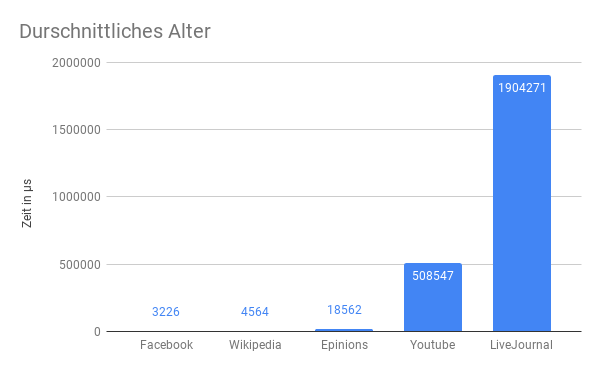
\includegraphics[width=\textwidth]{images/DurschAlter.png}
	\caption{Messergebnisse zur Berechnung des Durchschnittsalter}
	\label{fig:DurschAlter}
\end{figure}

\begin{figure}
	\centering
	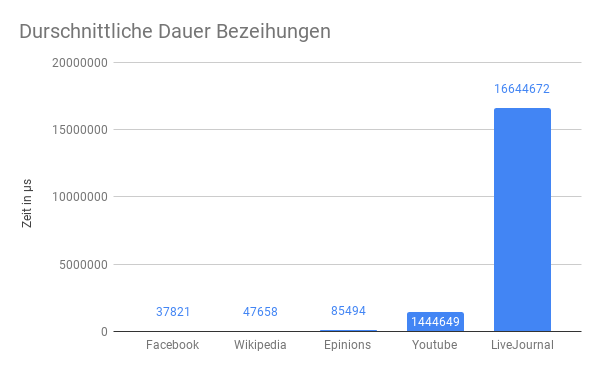
\includegraphics[width=\textwidth]{images/DurschBeziehung.png}
	\caption{Messergebnisse zur Berechnung der Dauer eine durchschnittlichen Beziehung}
	\label{fig:DurschBeziehung}
\end{figure}

\newpage

\subsubsection{Traversierung}
Für die Traversierung wird OQGRAPH-Engine verwendet, aber zuerst für Benutzung der OQGRAPH werden spezialle Vorbereitungstabellen erstellt, bei dessen Aufbau nur die relationalen Befehlen durchgeführt wurden.

Folgende Tests wurden durchgeführt:
\begin{enumerate}
	\item Erstellung der OQGRAPH Tabellen \ref{fig:facevor}
	\ref{fig:wikivor}
	\ref{fig:epinvor}
	\ref{fig:youtubvor}
	\ref{fig:LiJouvor}
	\item Transitive Suche in Facebook
	\ref{fig:face}
	\item Transitive Suche in Wikipedia
	\ref{fig:wiki}
	\item Transitive Suche in Epinions 
	\ref{fig:epin}
	\item Transitive Suche in Youtube 
	\ref{fig:youtub}
	\item Transitive Suche in LiveJournal 
	\ref{fig:LiJou}
\end{enumerate}


Folgende SQL Statements (nur die wichtige SQL Befehlen) wurden durchgeführt:
\begin{lstlisting}
-- Vorbereitung Tabelle der Business Kontakten
SELECT * FROM oq_backing WHERE rtype = "BUSINE";

-- Vorbereitung Tabelle der auslaendischen Kontakten
SET @land = 'BE';
SELECT DISTINCT * FROM 
(SELECT b1.origid, b1.destid FROM oq_backing b1 INNER JOIN
 profil p1 ON b1.destid = p1.id WHERE p1.country <> @land
UNION
SELECT b2.origid, b2.destid FROM oq_backing b2 INNER JOIN
 profil p2 ON b2.origid = p2.id WHERE p2.country <> @land
UNION
SELECT b3.origid, b3.destid FROM oq_backing b3 INNER JOIN
 profil p3 ON b3.origid = p3.id WHERE p3.id = sID
UNION
SELECT b4.origid, b4.destid FROM oq_backing b4 INNER JOIN
 profil p4 ON b4.destid = p4.id WHERE p4.id = sID);
 
-- Suche nach Kontakten
SELECT * FROM oq_graph WHERE latch='breadth_first' AND
 origid="start ID Knote" AND weight <= "Tiefe gerichtet" AND
  weight>0;
  
-- Suche nach Business Kontakten
SELECT * FROM oq_graph_business WHERE latch='breadth_first'
 AND origid="start ID Knote" AND weight <= "Tiefe gerichtet"
  AND weight>0;
  
-- Suche nach auslaendischen Kontakten
SELECT * FROM oq_graph_ausland WHERE latch='breadth_first'
 AND origid="start ID Knote" AND weight <= "Tiefe gerichtet"
  AND weight>0;
\end{lstlisting}


\begin{figure}
	\centering
	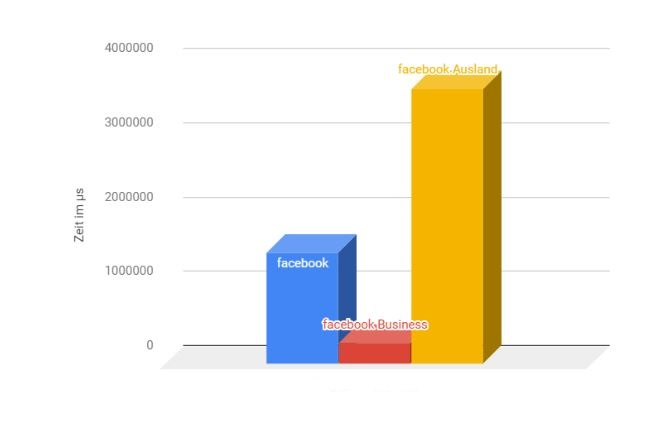
\includegraphics[width=\textwidth]{images/facevor.jpg}
	\caption{Messergebnisse zur Vorbereitung OQGRAPH Tabelle Facebook}
	\label{fig:facevor}
\end{figure}

\begin{figure}
	\centering
	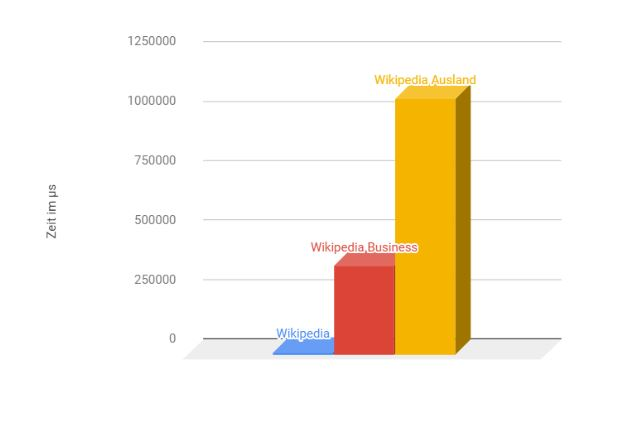
\includegraphics[width=\textwidth]{images/wikivor.jpg}
	\caption{Messergebnisse zur Vorbereitung OQGRAPH Tabelle Wikipedia}
	\label{fig:wikivor}
\end{figure}

\begin{figure}
	\centering
	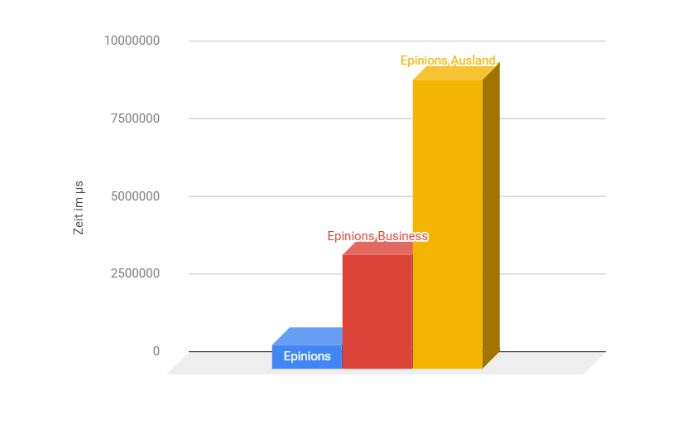
\includegraphics[width=\textwidth]{images/epinvor.jpg}
	\caption{Messergebnisse zur Vorbereitung OQGRAPH Tabelle Epinions}
	\label{fig:epinvor}
\end{figure}

\begin{figure}
	\centering
	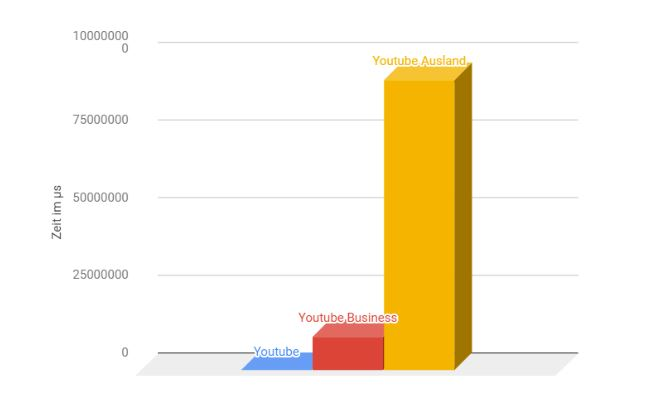
\includegraphics[width=\textwidth]{images/youtubvor.jpg}
	\caption{Messergebnisse zur Vorbereitung OQGRAPH Tabelle YouTube}
	\label{fig:youtubvor}
\end{figure}

\begin{figure}
	\centering
	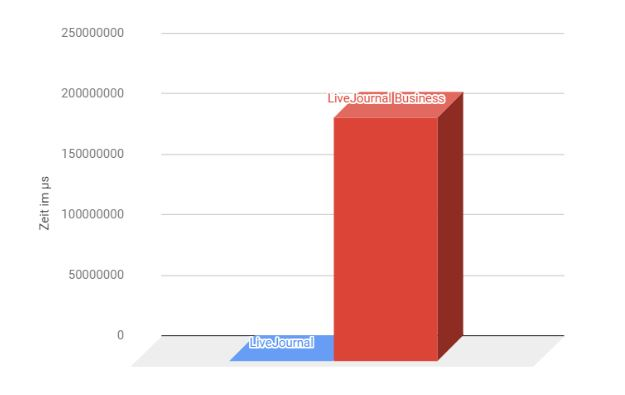
\includegraphics[width=\textwidth]{images/LiJouvor.jpg}
	\caption{Messergebnisse zur Vorbereitung OQGRAPH Tabelle LiveJournal}
	\label{fig:LiJouvor}
\end{figure}

Die Ergebnisse sind ganz erwarten, dass je größer die Datebanken sind, desto mehr die Zeit wird für die Erstellung der Tabellen benötigt und im Fall der QOGRAPH ausländischen Tabellen im LiveJournall ist Aufwand wegen mehreren JOIN Befehelen wirklich zu groß um die Ergebnisse zu berechnen.
Auch geht es um die kleine Daten im Tabelle "Facebook", darum kann die Tabelle manchmal  für die geschäftlichen Kontakten ein bisschen schneller erstellt werden.  


\begin{figure}
	\centering
	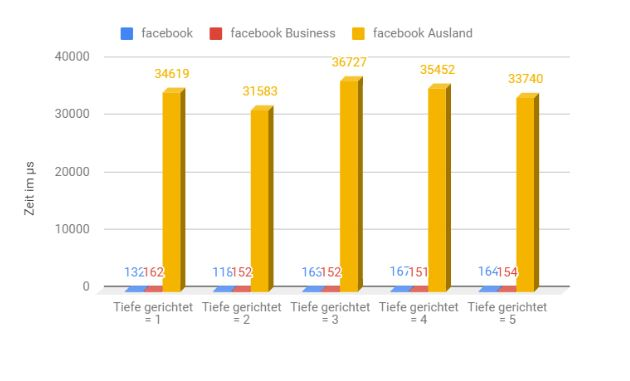
\includegraphics[width=\textwidth]{images/face.jpg}
	\caption{Messergebnisse nach Tiefenstufen in Tabelle Facebook}
	\label{fig:face}
\end{figure}

\begin{figure}
\centering
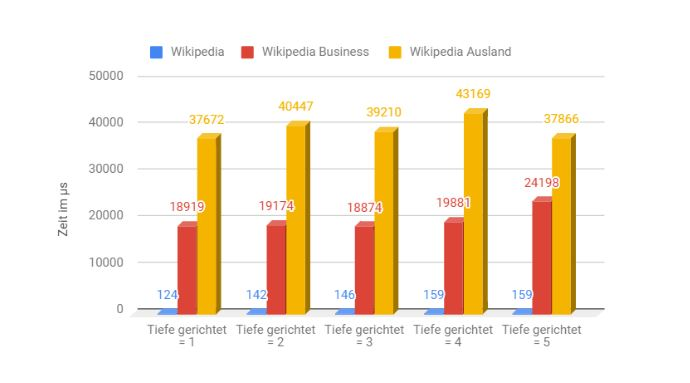
\includegraphics[width=\textwidth]{images/wiki.jpg}
\caption{Messergebnisse nach Tiefenstufen in Tabelle Wikipedia}
\label{fig:wiki}
\end{figure}

\begin{figure}
	\centering
	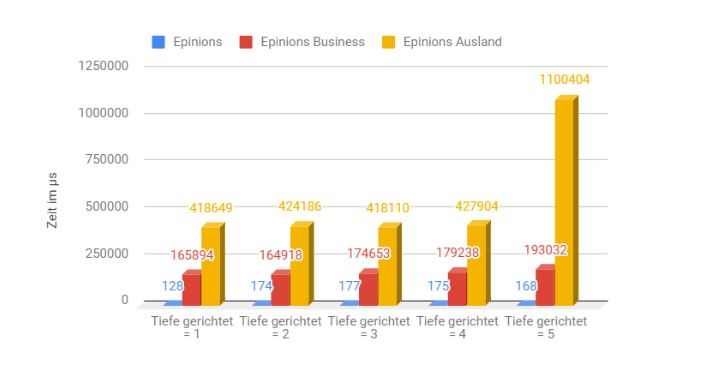
\includegraphics[width=\textwidth]{images/epin.jpg}
	\caption{Messergebnisse nach Tiefenstufen in Tabelle Epinions}
	\label{fig:epin}
\end{figure}

\begin{figure}
	\centering
	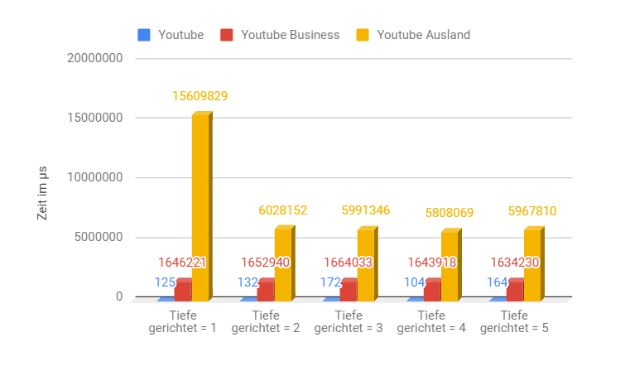
\includegraphics[width=\textwidth]{images/youtub.jpg}
	\caption{Messergebnisse nach Tiefenstufen in Tabelle YouTube}
	\label{fig:youtub}
\end{figure}

\begin{figure}
	\centering
	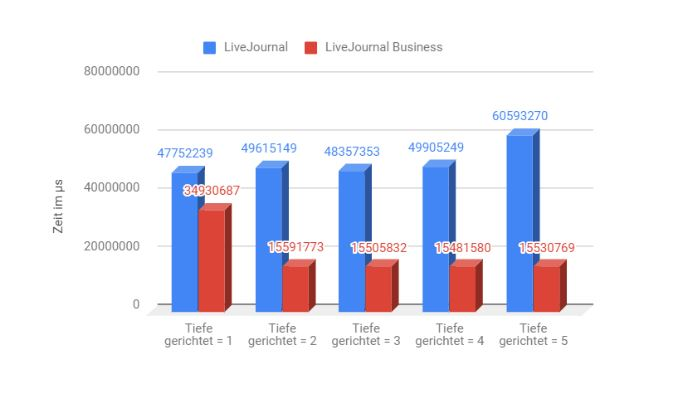
\includegraphics[width=\textwidth]{images/LiJou.jpg}
	\caption{Messergebnisse nach Tiefenstufen in Tabelle LiveJournal}
	\label{fig:LiJou}
\end{figure}

Allgemeine kann man feststellen, dass die Bearbeitungszeit für jede Transitive Suche vom Tiefstufen unabhängig ist. Manchmal ist bei einigen Suchen die Bearbeitungszeit groß,  z.B als auf dem Diagramm der Epinions im Tiefestufe 5, aber manchmal ist es auch in der Tiefestufe 1 auch, als in Youtube, darum hängt die Bearbeitungszeit von etwas Anderes als Tiefstufen ab. Und trotz vielen Zahlen der Knoten im Livejournal bleibt diese Tendenz fast gleich.

\subsection{Fazit}
Ebenso wie bei der OLTP Anwendung erfordert der begrenzte Funktionsumfang von OQGRAPH ein Ausweichen auf relationales SQL. Lediglich bei der Traversierung von Knoten kamen Funktionalitäten von OQGRAPH zum Einsatz, allerdings musste auch hier mit Workarounds gearbeitet werden um die Limitierung der homogenen Kanten zu umgehen. Die Performance selbst kann dabei mit konkurrierenden Graphdatenbanken mithalten. Positiv bemerkbar hat sich das koexistierende relationale Datenmodel hingegen bei der Aggregation gemacht, hier kamen die Vorteile von SQL zum Einsatz.